\chapter{Chemical Kinetics: Rate Laws}\label{ch:b1:rate-laws}

Milk keeps a week in the refrigerator and a day on a summer table. The
box of a medicine says ``store below \qty{25}{\celsius}'' and carries an
expiry date two or three years ahead, which the manufacturer had no time
to observe directly. Equilibrium constants say where a reaction ends;
they say nothing of how long it takes to get there. That is the domain of
chemical kinetics. This chapter defines the rate of a reaction, the \omterm{def:b1:rate-laws:order}{rate
laws} that express it in terms of concentrations, the integrated forms
that predict concentrations at any time, the experimental methods that
determine a \omterm{def:b1:rate-laws:order}{rate law}, and the \omterm{thm:b1:rate-laws:arrhenius}{Arrhenius law} that describes the effect of
temperature --- the tool by which the shelf life of a medicine is
predicted in a few weeks of experiments.

\begin{recall}
Book 1 (grade 12) introduced the rate of appearance and disappearance of
a species, the kinetic factors (concentration, temperature, catalyst) and
the \omterm{def:b1:rate-laws:half-life}{half-life} of a first-order reaction. The extent $\xi$ of a reaction
was defined in \cref{def:b1:extent-q-and-k:extent}.
\end{recall}

\begin{omfigure}
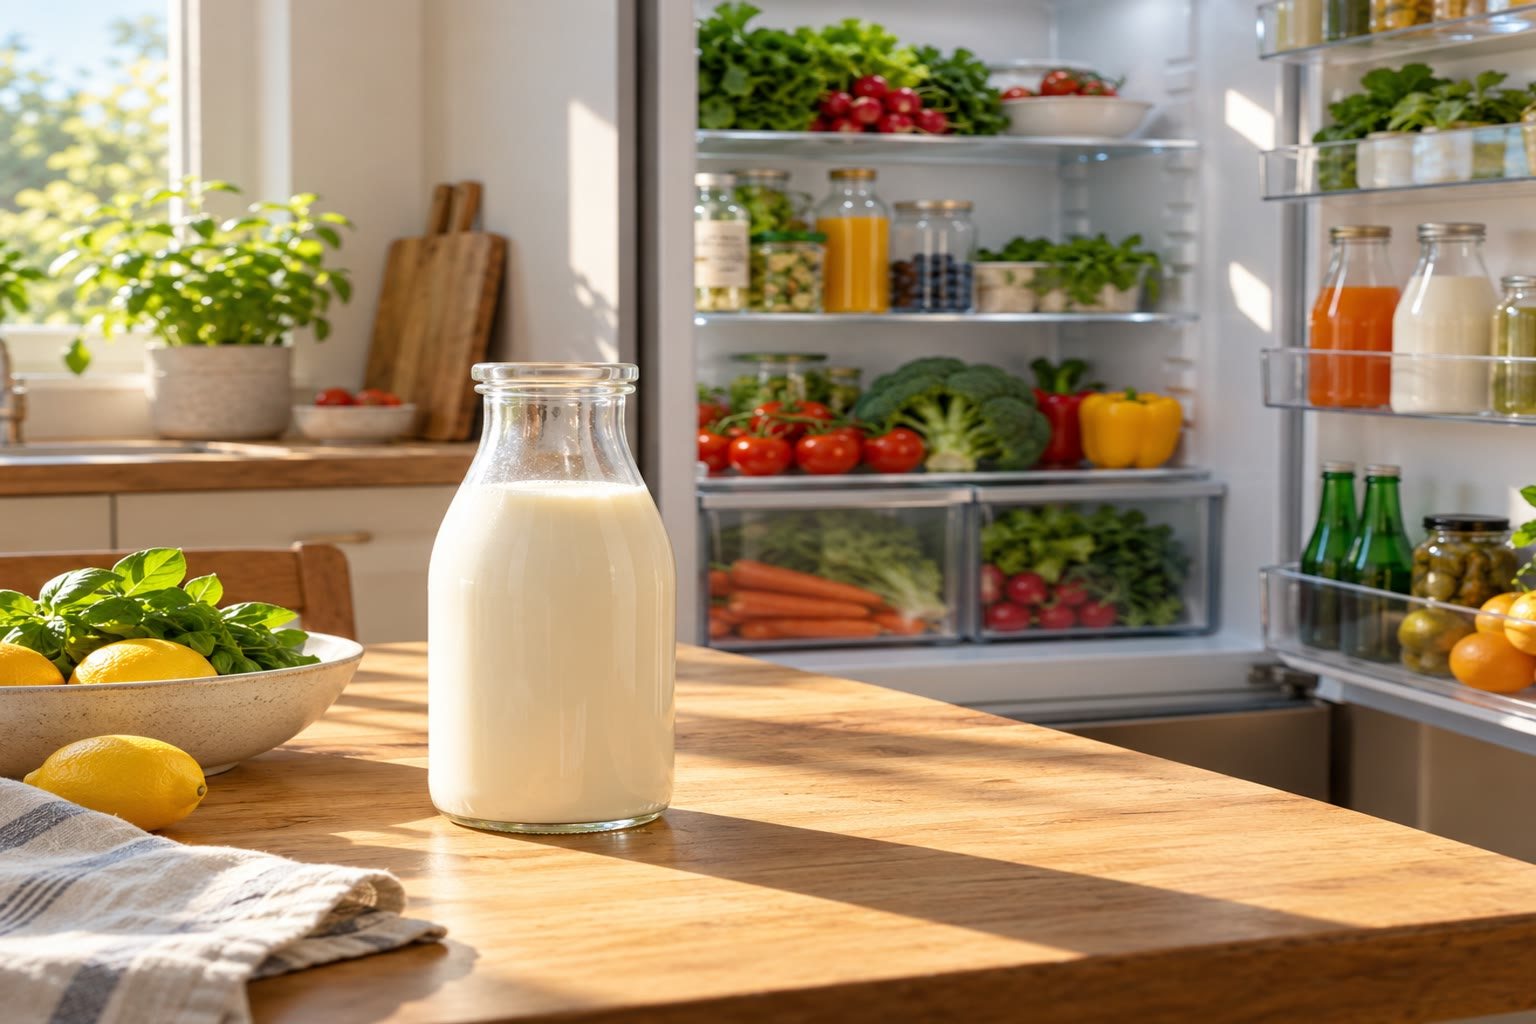
\includegraphics[width=0.55\linewidth]{images/book2/ai/b1-08-milk-kitchen.jpg}

{\small A bottle of milk left in the sun next to an open refrigerator.
The reactions that spoil it go several times faster at summer
temperature than in the cold.}
\end{omfigure}

\section{The rate of a reaction}

\begin{definition}[Rate of reaction, rates of formation and disappearance]\label{def:b1:rate-laws:rate}
For a reaction $0 = \sum_i \nu_i\mathrm{A}_i$ taking place in a closed
reactor of constant volume $V$, the \emph{rate of reaction}\index{rate of reaction}
is
\[
  v = \frac{1}{V}\frac{\dd\xi}{\dd t} = \frac{1}{\nu_i}\frac{\dd[\mathrm{A}_i]}{\dd t}
  \quad\text{(any } i\text{)},
\]
in \unit{mol.L^{-1}.s^{-1}}. The \emph{rate of formation}\index{rate of formation}
of a product is $\dd[\mathrm{A}_i]/\dd t$; the \emph{rate of
disappearance}\index{rate of disappearance} of a reactant is
$-\dd[\mathrm{A}_i]/\dd t$.
\end{definition}

\begin{proposition}[One rate for all species]\label{prop:b1:rate-laws:rate-relations}
The \omterm{def:b1:rate-laws:rate}{rate of reaction} does not depend on the species chosen to follow it:
for $a\,\mathrm{A} + b\,\mathrm{B} \longrightarrow c\,\mathrm{C} + d\,\mathrm{D}$,
\[
  v = -\frac1a\frac{\dd[\ce{A}]}{\dd t} = -\frac1b\frac{\dd[\ce{B}]}{\dd t}
  = \frac1c\frac{\dd[\ce{C}]}{\dd t} = \frac1d\frac{\dd[\ce{D}]}{\dd t} .
\]
\end{proposition}

\begin{proof}
$[\mathrm{A}_i] = (n_{i,0} + \nu_i\xi)/V$ with $V$ constant, so
$\dd[\mathrm{A}_i]/\dd t = (\nu_i/V)\,\dd\xi/\dd t = \nu_i v$.
\end{proof}

\begin{example}[Decomposition of dinitrogen pentoxide]\label{ex:b1:rate-laws:n2o5}
For \ce{2N2O5 -> 4NO2 + O2}: $v = -\frac12\frac{\dd[\ce{N2O5}]}{\dd t} =
\frac14\frac{\dd[\ce{NO2}]}{\dd t} = \frac{\dd[\ce{O2}]}{\dd t}$. Nitrogen
dioxide appears four times as fast as dioxygen, and dinitrogen pentoxide
disappears twice as fast as dioxygen appears.
\end{example}

\section{Rate laws and orders}

\begin{definition}[Rate law, orders, rate constant]\label{def:b1:rate-laws:order}
A \emph{rate law}\index{rate law} expresses the rate as a function of the
concentrations. A reaction \emph{has an order} when its rate law takes the
form
\[
  v = k\,[\mathrm{A}]^{p}\,[\mathrm{B}]^{q} \cdots ;
\]
the exponents $p$, $q$, \dots\ are the \emph{partial orders}\index{partial order}
with respect to A, B, \dots, their sum is the \emph{overall
order}\index{overall order}, and $k$ is the \emph{rate constant}\index{rate constant},
which depends on temperature only. Orders are found by
experiment; they need not equal the stoichiometric coefficients, and they
can be fractional or zero.
\end{definition}

\begin{remark}[Units of $k$]\label{rem:b1:rate-laws:units}
Since $v$ is in \unit{mol.L^{-1}.s^{-1}}, $k$ is in
\unit{mol.L^{-1}.s^{-1}} for order 0, \unit{s^{-1}} for order 1,
\unit{L.mol^{-1}.s^{-1}} for order 2, and in general
$(\unit{mol/L})^{1-n}\,\unit{s^{-1}}$ for \omterm{def:b1:rate-laws:order}{overall order} $n$. The unit of
$k$ tells the \omterm{def:b1:rate-laws:order}{overall order}.
\end{remark}

\begin{remark}[Reactions without order]\label{rem:b1:rate-laws:no-order}
Not every reaction has an order. The rate of some reactions is a fraction
whose denominator contains concentrations, or depends on the
concentration of a product. Such \omterm{def:b1:rate-laws:order}{rate laws} are explained by the
mechanism of the reaction (\cref{ch:b1:elementary-steps}). A reaction
may also have an order at the beginning only: the \omterm{def:b1:rate-laws:initial-rate}{initial rate} law.
\end{remark}

\section{Integrated rate laws and half-lives}

\begin{definition}[Half-life]\label{def:b1:rate-laws:half-life}
The \emph{half-life}\index{half-life} $t_{1/2}$ of a reactant is the time
after which half of its initial amount has been consumed.
\end{definition}

\begin{theorem}[Integrated rate laws]\label{thm:b1:rate-laws:integrated}
For a reaction $a\mathrm{A} \rightarrow \text{products}$ of rate $v = -\frac1a\frac{\dd[\ce{A}]}
{\dd t} = k[\ce{A}]^n$, with $[\ce{A}](0) = a_0$:
\begin{center}
\begin{tabular}{llll}
\hline
order & integrated law & linear plot & \omterm{def:b1:rate-laws:half-life}{half-life} \\
\hline
0 & $[\ce{A}] = a_0 - akt$ & $[\ce{A}]$ against $t$ & $a_0/(2ak)$ \\
1 & $[\ce{A}] = a_0\,\eu^{-akt}$ & $\ln[\ce{A}]$ against $t$ & $\ln2/(ak)$ \\
2 & $\dfrac{1}{[\ce{A}]} = \dfrac{1}{a_0} + akt$ & $1/[\ce{A}]$ against $t$ & $1/(ak\,a_0)$ \\
\hline
\end{tabular}
\end{center}
\end{theorem}

\begin{proof}
Write $c = [\ce{A}]$, so $\dd c/\dd t = -akc^n$.
\emph{Order 0}: $\dd c/\dd t = -ak$, hence $c = a_0 - akt$ (valid until
$c = 0$). \emph{Order 1}: $\dd c/\dd t = -akc$ is a first-order linear
differential equation whose solution is $c = a_0\eu^{-akt}$.
\emph{Order 2}: $\dd c/c^2 = -ak\,\dd t$; integrating from 0 to $t$,
$-1/c + 1/a_0 = -akt$, so $1/c = 1/a_0 + akt$. Half-lives: set $c =
a_0/2$ in each law and solve for $t$.
\end{proof}

\begin{proposition}[The half-life test]\label{prop:b1:rate-laws:half-life-test}
The \omterm{def:b1:rate-laws:half-life}{half-life} is independent of the initial concentration if and only if
the reaction is of order 1. It is proportional to $a_0$ for order 0 and
to $1/a_0$ for order 2. A first-order reaction loses half of what is left
in each successive \omterm{def:b1:rate-laws:half-life}{half-life}: after $m$ half-lives a fraction $2^{-m}$
remains.
\end{proposition}

\begin{proof}
For order $n \ne 1$, separating variables gives $t_{1/2} = \dfrac{2^{n-1} -
1}{(n-1)\,ak\,a_0^{n-1}}$, which depends on $a_0$ unless $n = 1$; for
$n = 1$, $t_{1/2} = \ln2/(ak)$. For order 1, $c(t + t_{1/2}) = c(t)/2$ at
every $t$, since $\eu^{-ak(t + t_{1/2})} = \eu^{-akt}/2$.
\end{proof}

\begin{omfigure}
\begin{tikzpicture}
\begin{axis}[name=p0,
  width=0.36\linewidth, height=4.6cm,
  xmin=0, xmax=60, ymin=0, ymax=1.05,
  axis x line=bottom, axis y line=left,
  xlabel={$t$ (min)}, title={order 0: $[\ce{A}]$},
  title style={font=\small}, xtick={0,20,40,60},
  tick label style={font=\scriptsize}, label style={font=\small}]
\addplot[omDef, thick] table[x=t, y=A0] {figdata/out/bachelor-1-integrated-rate-laws.dat};
\end{axis}
\begin{axis}[at={(p0.east)}, anchor=west, xshift=0.9cm, name=p1,
  width=0.36\linewidth, height=4.6cm,
  xmin=0, xmax=60, ymin=-3.2, ymax=0.2,
  axis x line=bottom, axis y line=left,
  xlabel={$t$ (min)}, title={order 1: $\ln[\ce{A}]$},
  title style={font=\small}, xtick={0,20,40,60},
  tick label style={font=\scriptsize}, label style={font=\small}]
\addplot[omProp, thick] table[x=t, y=lnA1] {figdata/out/bachelor-1-integrated-rate-laws.dat};
\end{axis}
\begin{axis}[at={(p1.east)}, anchor=west, xshift=0.9cm,
  width=0.36\linewidth, height=4.6cm,
  xmin=0, xmax=60, ymin=0, ymax=4.2,
  axis x line=bottom, axis y line=left,
  xlabel={$t$ (min)}, title={order 2: $1/[\ce{A}]$},
  title style={font=\small}, xtick={0,20,40,60},
  tick label style={font=\scriptsize}, label style={font=\small}]
\addplot[omThm, thick] table[x=t, y=invA2] {figdata/out/bachelor-1-integrated-rate-laws.dat};
\end{axis}
\end{tikzpicture}

\begin{tikzpicture}
\begin{axis}[
  width=0.62\linewidth, height=5.0cm,
  xmin=0, xmax=60, ymin=0, ymax=1.05,
  axis x line=bottom, axis y line=left,
  xlabel={$t$ (min)}, ylabel={$[\ce{A}]$ (mol/L)}, xtick={0,10,20,30,40,50,60},
  tick label style={font=\small}, label style={font=\small},
  legend style={font=\small, draw=none, at={(0.98,0.98)}, anchor=north east}]
\addplot[omDef, thick] table[x=t, y=A0] {figdata/out/bachelor-1-integrated-rate-laws.dat};
\addplot[omProp, thick] table[x=t, y=A1] {figdata/out/bachelor-1-integrated-rate-laws.dat};
\addplot[omThm, thick] table[x=t, y=A2] {figdata/out/bachelor-1-integrated-rate-laws.dat};
\legend{order 0, order 1, order 2}
\draw[dotted] (axis cs:0,0.5) -- (axis cs:20,0.5);
\end{axis}
\end{tikzpicture}

{\small Three reactions with the same initial concentration
(\qty{1.00}{mol/L}) and the same \omterm{def:b1:rate-laws:initial-rate}{initial rate}
(\qty{0.050}{mol.L^{-1}.min^{-1}}). Top: each integrated law becomes a
straight line in its own coordinates. Bottom: the concentrations; the
half-lives are 10, 13.9 and 20 minutes.}
\end{omfigure}

\section{Finding a rate law}

\begin{method}[The integral method]\label{met:b1:rate-laws:integral}
To test an order with measurements $[\ce{A}](t)$: plot $[\ce{A}]$,
$\ln[\ce{A}]$ and $1/[\ce{A}]$ against $t$; the plot that is a straight
line gives the order, and its slope gives $k$ (slope $-ak$, $-ak$ or $+ak$
respectively).
\end{method}

\begin{method}[The half-life method]\label{met:b1:rate-laws:half-life}
Measure the \omterm{def:b1:rate-laws:half-life}{half-life} for several initial concentrations: constant,
order 1; proportional to $a_0$, order 0; proportional to $1/a_0$, order
2. In a single experiment, compare the times to go from $a_0$ to $a_0/2$
and from $a_0/2$ to $a_0/4$: equal times mean order 1.
\end{method}

\begin{definition}[Initial rate]\label{def:b1:rate-laws:initial-rate}
The \emph{initial rate}\index{initial rate} $v_0$ is the rate at $t = 0$,
read as the slope of the tangent at the origin of the curve $[\ce{A}](t)$,
divided by the stoichiometric coefficient. At that moment the
concentrations are the known initial ones and no product interferes.
\end{definition}

\begin{method}[The method of initial rates]\label{met:b1:rate-laws:initial-rates}
For $v_0 = k[\ce{A}]_0^p[\ce{B}]_0^q$: run experiments that change
$[\ce{A}]_0$ alone; then $\ln v_0 = \ln(k[\ce{B}]_0^q) + p\ln[\ce{A}]_0$,
and the slope of $\ln v_0$ against $\ln[\ce{A}]_0$ is $p$. In practice,
doubling $[\ce{A}]_0$ multiplies $v_0$ by $2^p$. Do the same for B.
\end{method}

\begin{definition}[Isolation method, apparent order]\label{def:b1:rate-laws:apparent-order}
In the \emph{isolation method}\index{isolation method}, all reactants but
one are put in large excess (ten times or more). Their concentrations stay
practically constant, and $v = k[\ce{A}]^p[\ce{B}]^q \approx k'[\ce{A}]^p$
with $k' = k[\ce{B}]_0^q$: the reaction behaves as if of
\emph{apparent order}\index{apparent order} $p$ with the apparent \omterm{def:b1:rate-laws:order}{rate
constant} $k'$. This is also called degeneracy of the order.
\end{definition}

\begin{omfigure}
\begin{tikzpicture}
\begin{axis}[
  width=0.55\linewidth, height=4.8cm,
  xmin=0, xmax=40, ymin=0, ymax=1.05,
  axis x line=bottom, axis y line=left,
  xlabel={$t$ (min)}, ylabel={$[\ce{A}]$ (mol/L)},
  xtick={0,10,20,30,40},
  tick label style={font=\small}, label style={font=\small}, clip mode=individual]
\addplot[omProp, thick] table[x=t, y=A1] {figdata/out/bachelor-1-integrated-rate-laws.dat};
\draw[omThm, thick] (axis cs:0,1) -- (axis cs:20,0);
\node[omThm, anchor=west, font=\small] at (axis cs:2,0.12) {tangent at $t = 0$};
\end{axis}
\end{tikzpicture}

{\small Reading an \omterm{def:b1:rate-laws:initial-rate}{initial rate}: the tangent at the origin (red) of a
first-order curve meets the time axis at $t_0 = \qty{20}{min}$, so $v_0 =
\qty{1.00}{mol/L}/\qty{20}{min} = \qty{0.050}{mol.L^{-1}.min^{-1}}$.}
\end{omfigure}

\begin{inthelab}[Following a reaction in time]
A \omterm{def:b1:rate-laws:order}{rate law} is built from concentrations measured while the reaction runs.
When a reactant or a product is coloured, a spectrophotometer records the
absorbance, proportional to its concentration (Beer--Lambert,
\cref{ch:b1:structure-spectroscopy}); when ions appear or disappear, a
conductimeter follows the conductivity; when a gas forms in a closed
vessel, a manometer follows the pressure. Otherwise samples are taken at
known times, the reaction is stopped (quenched) by cooling or dilution,
and each sample is titrated. The temperature of the vessel is held
constant by a thermostatic bath, because $k$ depends strongly on it.
\end{inthelab}

\section{Temperature: the Arrhenius law}

\begin{definition}[Activation energy]\label{def:b1:rate-laws:activation-energy}
The \emph{activation energy}\index{activation energy} $E_a$ of a reaction
of \omterm{def:b1:rate-laws:order}{rate constant} $k(T)$ is defined by
\[
  \frac{\dd \ln k}{\dd T} = \frac{E_a}{RT^2} ,
\]
in \unit{J/mol}. When $E_a$ is independent of $T$, integrating gives
$k = A\,\eu^{-E_a/RT}$, where the constant $A$, of the unit of $k$, is the
\emph{pre-exponential factor}\index{pre-exponential factor}.
\end{definition}

\begin{theorem}[Arrhenius law]\label{thm:b1:rate-laws:arrhenius}
For most reactions, over a moderate range of temperature, the \omterm{def:b1:rate-laws:order}{rate
constant} follows the \emph{Arrhenius law}\index{Arrhenius law}
\[
  k(T) = A\,\eu^{-E_a/RT} ,
\]
with $A$ and $E_a > 0$ independent of $T$: $\ln k$ is a linear function of
$1/T$ of slope $-E_a/R$.
\end{theorem}
\admitted

\begin{remark}[The meaning of $E_a$]\label{rem:b1:rate-laws:meaning}
The law is empirical. Its interpretation --- only the molecular collisions
that carry at least an energy of the order of $E_a$ lead to reaction, and
the fraction of such collisions varies as $\eu^{-E_a/RT}$ --- is sketched
with the energy profiles of the next chapter and made quantitative by the
theories of reaction rates in the Year 3 volume.
\end{remark}

\begin{method}[Determining $E_a$]\label{met:b1:rate-laws:arrhenius-plot}
From \omterm{def:b1:rate-laws:order}{rate constants} at several temperatures, plot $\ln k$ against $1/T$
(in kelvin): the slope is $-E_a/R$, the intercept $\ln A$. With two
temperatures only,
\[
  E_a = \frac{R\,\ln(k_2/k_1)}{1/T_1 - 1/T_2} .
\]
\end{method}

\begin{example}[A rule of thumb]\label{ex:b1:rate-laws:doubling}
For $E_a = \qty{53}{kJ/mol}$, going from 25 to \qty{35}{\celsius}
multiplies $k$ by $\exp\!\big(\frac{53000}{8.314}(\frac{1}{298.15} -
\frac{1}{308.15})\big) = 2.0$. The familiar rule ``ten degrees more, twice
as fast'' holds near room temperature for reactions of \omterm{def:b1:rate-laws:activation-energy}{activation energy}
around \qty{50}{kJ/mol}; for larger $E_a$ the factor is larger.
\end{example}

\begin{omfigure}
\begin{tikzpicture}
\begin{axis}[
  width=0.6\linewidth, height=5.4cm,
  xmin=2.95, xmax=3.45, ymin=-9.0, ymax=-4.2, clip mode=individual,
  axis x line=bottom, axis y line=left,
  xlabel={$1000/T$ (\unit{K^{-1}})}, ylabel={$\ln k$ ($k$ in \unit{d^{-1}})},
  xtick={3.0,3.1,3.2,3.3,3.4}, ytick={-9,-8,-7,-6,-5},
  tick label style={font=\small}, label style={font=\small}]
\addplot[omDef, thick] table[x=invT_1e3, y=lnk] {figdata/out/bachelor-1-arrhenius-line.dat};
\addplot[only marks, mark=*, mark size=2.2pt, omThm] table[x=invT_1e3, y=lnk] {figdata/out/bachelor-1-arrhenius-points.dat};
\node[font=\small, anchor=south west] at (axis cs:3.002,-4.71) {\qty{60}{\celsius}};
\node[font=\small, anchor=south west] at (axis cs:3.095,-5.66) {\qty{50}{\celsius}};
\node[font=\small, anchor=south west] at (axis cs:3.193,-6.67) {\qty{40}{\celsius}};
\draw[dashed, black!50] (axis cs:3.354,-9.0) -- (axis cs:3.354,-8.31);
\addplot[only marks, mark=o, mark size=2.4pt, omDef] coordinates {(3.354,-8.310)};
\node[font=\small, anchor=east] at (axis cs:3.33,-8.40) {\qty{25}{\celsius}, extrapolated};
\end{axis}
\end{tikzpicture}

{\small Arrhenius plot of the degradation of a medicine (weekend
problem): three measured \omterm{def:b1:rate-laws:order}{rate constants} (red) lie on a line of slope
$-E_a/R$; extrapolated to \qty{25}{\celsius}, it gives the shelf life at
room temperature.}
\end{omfigure}

\begin{history}[Arrhenius, 1889]
The Swedish chemist Svante Arrhenius, studying the inversion of sucrose by
acids in 1889, proposed that only a small fraction of the molecules, those
in an ``activated'' state, react, and that this fraction grows with
temperature as $\eu^{-E/RT}$. The idea, controversial at first, became the
foundation of chemical kinetics. Arrhenius received the Nobel Prize in
Chemistry in 1903, for his theory of electrolytic dissociation.
\end{history}

\begin{omfigure}
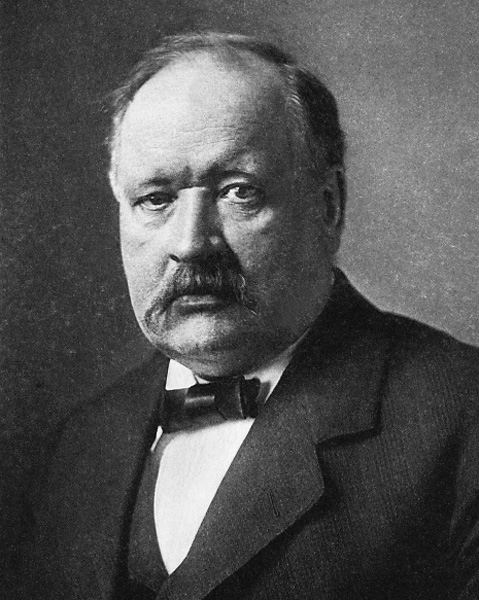
\includegraphics[width=0.22\linewidth]{images/book2/arrhenius.jpg}

{\small Svante Arrhenius (1859--1927), in 1909.}
\end{omfigure}

\section{Exercises}

\begin{exercise}[$\star$]\label{exo:b1:rate-laws:1}
For \ce{2N2O5 -> 4NO2 + O2} at constant volume, nitrogen dioxide appears at
$\qty{2.0e-4}{mol.L^{-1}.s^{-1}}$. Give the \omterm{def:b1:rate-laws:rate}{rate of reaction}, the \omterm{def:b1:rate-laws:rate}{rate of
formation} of dioxygen and the \omterm{def:b1:rate-laws:rate}{rate of disappearance} of \ce{N2O5}.
\end{exercise}

\begin{exercise}[$\star$]\label{exo:b1:rate-laws:2}
Give the unit of the \omterm{def:b1:rate-laws:order}{rate constant} for \omterm{def:b1:rate-laws:order}{overall orders} 0, 1, 2 and 3,
concentrations in \unit{mol/L} and times in seconds.
\end{exercise}

\begin{exercise}[$\star$]\label{exo:b1:rate-laws:3}
A first-order reaction $\mathrm{A} \longrightarrow \mathrm{B}$ has $k = \qty{3.0e-3}{s^{-1}}$. Compute
its \omterm{def:b1:rate-laws:half-life}{half-life} and the fraction of \ce{A} left after \qty{10}{min}.
\end{exercise}

\begin{exercise}[$\star$]\label{exo:b1:rate-laws:4}
When the initial concentration of a reactant is halved, its \omterm{def:b1:rate-laws:half-life}{half-life}
doubles. What is the order? What if the \omterm{def:b1:rate-laws:half-life}{half-life} is halved?
\end{exercise}

\begin{exercise}[$\star\star$]\label{exo:b1:rate-laws:5}
The concentration of a reactant \ce{A} ($\mathrm{A} \longrightarrow \mathrm{P}$) is measured: at $t
= 0$, 10, 20, 30 and \qty{40}{min}, $[\ce{A}] = 0.100$, 0.0741, 0.0549,
0.0407 and \qty{0.0301}{mol/L}. Determine the order and the \omterm{def:b1:rate-laws:order}{rate
constant}.
\end{exercise}

\begin{exercise}[$\star\star$]\label{exo:b1:rate-laws:6}
For $\mathrm{A} + \mathrm{B} \longrightarrow \mathrm{P}$, $v_0 = \qty{2.0e-6}{mol.L^{-1}.s^{-1}}$ for $[\ce{A}]_0
= [\ce{B}]_0 = \qty{0.010}{mol/L}$; \qty{8.0e-6}{} when $[\ce{A}]_0$ is
doubled; \qty{4.0e-6}{} when $[\ce{B}]_0$ is doubled. Find the \omterm{def:b1:rate-laws:order}{partial
orders}, the \omterm{def:b1:rate-laws:order}{rate law} and the \omterm{def:b1:rate-laws:order}{rate constant}.
\end{exercise}

\begin{exercise}[$\star\star$]\label{exo:b1:rate-laws:7}
The \omterm{def:b1:rate-laws:order}{rate law} of $\mathrm{A} + \mathrm{B} \longrightarrow \mathrm{P}$ is $v = k[\ce{A}][\ce{B}]$. With
$[\ce{B}]_0 = \qty{0.50}{mol/L}$ and $[\ce{A}]_0 = \qty{5.0e-3}{mol/L}$,
\ce{A} disappears with first-order kinetics and an apparent constant of
\qty{0.012}{s^{-1}}. Explain and compute $k$.
\end{exercise}

\begin{exercise}[$\star\star$]\label{exo:b1:rate-laws:8}
A \omterm{def:b1:rate-laws:order}{rate constant} is \qty{1.0e-3}{s^{-1}} at \qty{300}{K} and
\qty{5.0e-3}{s^{-1}} at \qty{320}{K}. Compute the \omterm{def:b1:rate-laws:activation-energy}{activation energy} and
the \omterm{def:b1:rate-laws:order}{rate constant} at \qty{310}{K}.
\end{exercise}

\begin{exercise}[$\star\star$]\label{exo:b1:rate-laws:9}
The reaction $2\,\mathrm{A} \longrightarrow \mathrm{P}$ has the \omterm{def:b1:rate-laws:order}{rate law} $v = -\frac12\frac{\dd[\ce{A}]}
{\dd t} = k[\ce{A}]^2$ with $k = \qty{0.50}{L.mol^{-1}.s^{-1}}$. Starting
from $[\ce{A}]_0 = \qty{0.020}{mol/L}$, compute the \omterm{def:b1:rate-laws:half-life}{half-life} and the
concentration after \qty{100}{s}.
\end{exercise}

\begin{exercise}[$\star\star\star$]\label{exo:b1:rate-laws:10}
For a first-order reaction, show that the time needed to consume a
fraction $f$ of the reactant is $t_f = -\ln(1 - f)/(ak)$. Compare the
times for 50\,\%, 75\,\%, 90\,\% and 99.9\,\%, in half-lives.
\end{exercise}

\begin{exercise}[$\star\star\star$]\label{exo:b1:rate-laws:11}
A skin patch releases a drug at a constant rate of
\qty{0.40}{mg/h} as long as its reservoir, initially \qty{10}{mg}, is not
empty. Write the law of the amount left, give its order, its \omterm{def:b1:rate-laws:half-life}{half-life} and
the time after which the patch is exhausted. Why do zero-order kinetics
suit a drug patch?
\end{exercise}

\begin{exercise}[$\star\star\star$]\label{exo:b1:rate-laws:12}
Show that the rule ``ten degrees more, twice as fast'' between
\qty{298.15}{K} and \qty{308.15}{K} corresponds to $E_a \approx
\qty{53}{kJ/mol}$. What factor does the same \omterm{def:b1:rate-laws:activation-energy}{activation energy} give
between \qty{0}{\celsius} and \qty{10}{\celsius}?
\end{exercise}

\section{Problem: The Shelf Life of a Medicine}

\begin{problem}[{Weekend problem --- an accelerated stability test:
first-order degradation at 60\,\textdegree C, three temperatures, the
Arrhenius plot, and the shelf life at room temperature}]
\label{pb:b1:rate-laws:1}
To predict the shelf life $t_{90}$ of a tablet (the time after which 10\,\%
of the active ingredient has degraded), a laboratory stores samples at
high temperature and measures the percentage of ingredient left. At
\qty{60}{\celsius}:
\begin{center}
\begin{tabular}{lccccc}
\hline
time (days) & 0 & 10 & 20 & 30 & 40 \\
ingredient left (\%) & 100.0 & 91.4 & 83.5 & 76.3 & 69.8 \\
\hline
\end{tabular}
\end{center}
At 40 and \qty{50}{\celsius} the \omterm{def:b1:rate-laws:order}{rate constants} found are
\qty{1.27e-3}{d^{-1}} and \qty{3.48e-3}{d^{-1}}. Take $R =
\qty{8.314}{J/(mol.K)}$ and one month $= \qty{30.4}{d}$.

\medskip
\noindent\textbf{Part I --- The order at 60\,\textdegree C.}
\begin{enumerate}
  \item Compute the losses over each 10-day interval. Is the reaction of
        order 0?
  \item Compute $\ln(\%\text{ left})$ at each time. What do you conclude?
  \item Deduce the \omterm{def:b1:rate-laws:order}{rate constant} $k_{60}$.
  \item Compute the \omterm{def:b1:rate-laws:half-life}{half-life} at \qty{60}{\celsius}.
  \item What percentage is left after 60 days at \qty{60}{\celsius}?
  \item Compute $t_{90}$ at \qty{60}{\celsius}.
\end{enumerate}

\medskip
\noindent\textbf{Part II --- Shelf life and order.}
\begin{enumerate}[resume]
  \item Show that for a first-order degradation $t_{90} = \ln(10/9)/k$.
  \item Express $t_{90}$ as a fraction of the \omterm{def:b1:rate-laws:half-life}{half-life}.
  \item Why does $t_{90}$ not depend on the dose of the tablet?
  \item Why do laboratories measure degradation at high temperature
        rather than at \qty{25}{\celsius}?
  \item If the degradation were of order 2 in the ingredient, would a
        tablet twice as strong keep longer or less long? Explain.
\end{enumerate}

\medskip
\noindent\textbf{Part III --- The Arrhenius plot.}
\begin{enumerate}[resume]
  \item Tabulate $1/T$ and $\ln k$ for the three temperatures.
  \item Compute the slope of the line through the 40 and
        \qty{60}{\celsius} points.
  \item Deduce the \omterm{def:b1:rate-laws:activation-energy}{activation energy}.
  \item Check that the \qty{50}{\celsius} point lies on the line.
  \item Compute the \omterm{def:b1:rate-laws:activation-energy}{pre-exponential factor} $A$.
  \item By what factor does the rate increase between 25 and
        \qty{35}{\celsius}? Compare with the rule of thumb.
\end{enumerate}

\medskip
\noindent\textbf{Part IV --- Room temperature.}
\begin{enumerate}[resume]
  \item Extrapolate the \omterm{def:b1:rate-laws:order}{rate constant} to \qty{30}{\celsius}.
  \item Compute $t_{90}$ at \qty{30}{\celsius}, in months.
  \item A box is forgotten three days in a car at \qty{60}{\celsius}. What
        fraction of the ingredient is lost?
  \item Explain the instruction ``store below \qty{25}{\celsius}''.
  \item Extrapolate the \omterm{def:b1:rate-laws:order}{rate constant} to \qty{25}{\celsius}.
  \item Compute the shelf life $t_{90}$ at \qty{25}{\celsius}, in days and
        in months.
\end{enumerate}
\end{problem}
